\chapter{Tests}

\section{Utilisation du client-serveur}

Nous nous proposons de tester notre implémentation. Nous allons essayer de nous connecter en ssh depuis le client sur le serveur applicatif ceci en utilisant la méthode SPA.

Nous allons depuis la machine client tenter une connexion ssh vers le serveur applicatif en 10.0.0.2

\begin{figure}[h]

\centerline{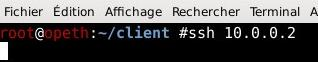
\includegraphics[scale=0.75]{test_ssh.jpeg}}

\end{figure}

Celle-ci ne fonctionne pas car les règles du pare-feu ne laissent pas passer la connexion.

\begin{figure}[h]

\centerline{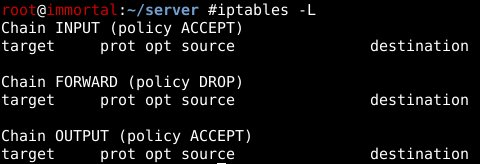
\includegraphics[scale=0.6]{regles_ip_avant}}

\end{figure}

Pour parrer à ces restrictions, nous allons envoyer un paquet SPA demandant de laisser passer les communications en tcp vers le port 22.

\begin{figure}[h]

\centerline{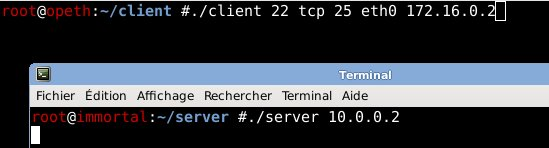
\includegraphics[scale=0.6]{execution_client.jpeg}}

\end{figure}

Voici ce que nous pouvons voir sur le serveur après réception du paquet.
\clearpage

\begin{figure}[h]

\centerline{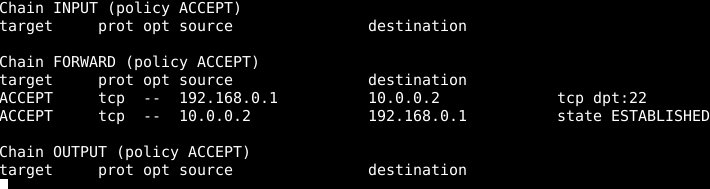
\includegraphics[scale=0.7]{regles_apres.jpeg}}

\end{figure}

La connexion ssh fonctionne maintenant (mais seulement pour le temps spécifié).

\begin{figure}[h]

\centerline{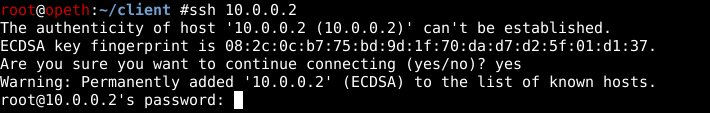
\includegraphics[scale=0.6]{test_ssh2.jpeg}}

\end{figure}

\clearpage
\section{Attaques}

Mettons-nous à la place de l'attaquant. En écoutant sur le réseau, nous retrouvons le paquet SPA formé de cette manière. On se rend compte que toutes les données sont chiffrées et qu'il n'y a que l'IV à la fin du message en clair.

\begin{figure}[h]

\centerline{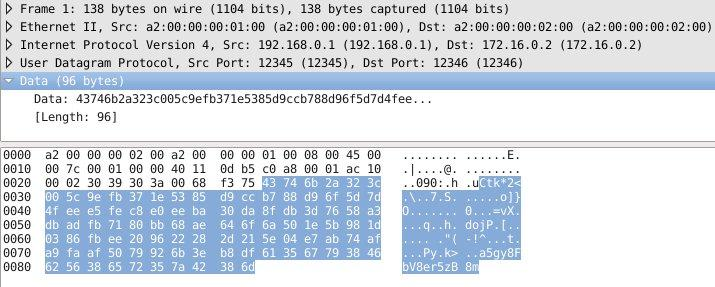
\includegraphics[scale=0.6]{wireshark.jpeg}}

\end{figure}

En essayant de rejouer un paquet sur le réseau, le serveur le détecte en n'en tient pas compte.

\begin{figure}[h]

\centerline{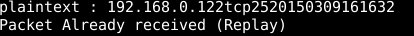
\includegraphics[scale=0.8]{rejeu.jpeg}}

\end{figure}

